\subtitle{Ecuación de transporte}
\begin{frame}
  \titlepage
\end{frame}
% Uncomment these lines for an automatically generated outline.
%\begin{frame}{Outline}
%  \tableofcontents
%\end{frame}

\section{Introducción}


\begin{frame}{Descripción del transporte}


Dos formas \textit{equivalentes} de pensar el problema: 
\begin{itemize}
    \item Descripción \alert{Lagrangiana} ó enfoque \textit{material}: Estudiar como se mueve un contaminante en el tiempo y espacio.
    
    \item Descripción \alert{Euleriana} ó enfoque de \textit{campos}: Estudiar como cambia con el tiempo la concentración de un contaminante en el espacio.
    
\end{itemize}

\begin{center}
    \includegraphics[width=0.6\textwidth]{img/MaterialDerivative.png}
\end{center}

En este curso vamos a adoptar la descripción \textbf{Euleriana}.
    
\end{frame}


%\begin{frame}{Representación del transporte}
%
%\begin{center}
%    
%\begin{tikzpicture}
%\begin{axis}[axis lines = empty]%center, ticks=none, axis on top, axis line style = {thick, black!80}]%[grid=both]
%    \addplot3[surf,fill=white, %shader=faceted interp,
%    samples=10, %point meta rel=per plot,
%    point meta={0}]{0};
%\end{axis}
%    \draw[-latex,ultra thick,blue!90] (2.5,4)--(4.5,4.2) node[above]{$u$};
%    \pause
%\begin{axis}[axis lines = center, ticks=none, axis on top, axis line style = {thick, black!80}]%[grid=both]
%    \addplot3[surf,
%    shader=faceted interp,
%    samples=10,point meta rel=per plot,
%    point meta={sin(deg(x))*sin(deg(y))+0.1*x+0.2*y}   
%    ] {0}; 
%\end{axis}
%\end{tikzpicture}
%\end{center}
%\end{frame}

\begin{frame}{Representación del transporte}

\textbf{Objetivo del curso:} Representar la concentración de un contaminante atmosférico (C) en el espacio y en el tiempo.\\[1em]

Podemos usar el concepto de \textit{función}:
\begin{center}
    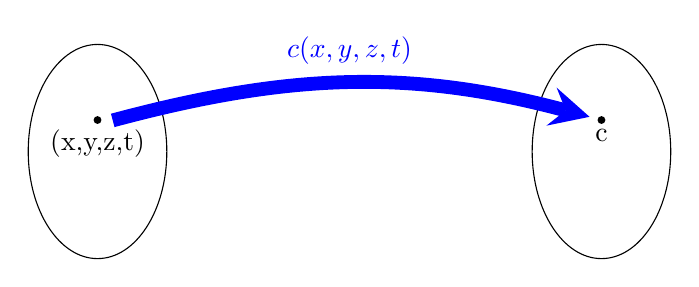
\begin{tikzpicture}[scale=0.8,
    >=stealth,
    bullet/.style={ fill=black, circle, minimum width=1pt, inner sep=1pt},
    every fit/.style={ ellipse, draw, inner sep=0pt }
    ]
    \node[bullet] (START) at (0,3){};
    \node[bullet] (END) at (8,3){};
    
    \node[anchor=north] at (START) {(x,y,z,t)};
    \node[anchor=north] at (END)  {c};
 
    \draw (0,2.5) ellipse (1.1cm and 1.7cm);
    \draw (8,2.5) ellipse (1.1cm and 1.7cm);
 
    \pause
    \draw [line width=5pt, blue, shorten <=0.2cm,, shorten >=0.1cm, ->] (START.south) to[out=15, in=165 ] (END);
    \node[blue] at (4,4.1){$c(x,y,z,t)$};

    \end{tikzpicture}
\end{center}
   
   
\end{frame}


 \begin{frame}{Ecuación de transporte}
\pause
Es una \textit{ecuación diferencial}\footnote{Ecuación cuya incógnita es una función} basada en el \textbf{principio de conservación de masa}.\\[2em]
\pause

Describe cómo cambia la concentración  de una especie química (C) en el tiempo para un punto del espacio.\\[2em]
%\item ¿Cómo? descripción \textbf{Euleriana} y \textbf{Lagrangiana}
\pause

Se deduce de analizar todos los procesos que generan un cambio en la concentración en un punto arbitrario del espacio.\\[2em]

%Objetivo:
%$$\boxed{\dfrac{\partial C}{\partial t} }$$
%%- ¿Porqué me interesaría saber esto?\\[1em]
% Si conocemos $C_t$ (condición inicial), y tenemos $\frac{\Delta C}{\Delta t}$ (Ecuación de transporte) entonces podemos predecir como va a ser C para algún tiempo futuro ($C_{t+1}$)\\[1em]
%%-¿Cómo? \\[1em] 
%%- Así:
%\pause
%  $$C_{t+1} = C_{t} + \dfrac{\Delta C}{\Delta t}$$
\end{frame}


\begin{frame}{}
    
\begin{tikzpicture}[remember picture, overlay]
    \node[opacity=1.,inner sep=1pt] (image) at (current page.center) {\includegraphics[height=\paperheight, width=1\paperwidth]{img/pollution_plumes.jpg}};
   \begin{scope}[x={(image.south east)},y={(image.north west)}]
        \pause
        \fill[red] (0.22,0.28) circle[radius=2pt] ++(0,0.06) node[anchor=south] {\textbf{Emisión}};
        \pause
        %Adveccion
        \draw[-stealth,ultra thick,blue] (0.4,0.7)--++(0.1,0.15) node[midway,anchor=north]{$\vec{u}$}node[midway,anchor=south]{\textbf{Advección}};
        \pause
        %Mezcla
        \draw[stealth-stealth,ultra thick,black!20!green] (0.6,0.85)--++(0.01,0.5)node[midway,anchor=west]{\textbf{Mezcla}};
        \pause
        %Quimica
        \draw[black!10!yellow] (0.8,0.9) node[anchor=south] {\textbf{Química}};
   \end{scope}
\end{tikzpicture}
\end{frame}
%






%% \begin{frame}{Objetivo}{Encontrar expresión matemática para $\Delta C/\Delta t$}
%%- ¿Cómo hacemos?\\[1em]
%\pause
%\begin{tikzpicture}
%    \node[anchor=south west,inner sep=0] (image) at (0,0) {\includegraphics[width=1\textwidth]{img/spersion-scheme.png}};
%   \begin{scope}[x={(image.south east)},y={(image.north west)}]
%        %\draw[red,help lines,xstep=.1,ystep=.1] (0,0) grid (1,1);
%        %\foreach \x in {0,1,...,9} { \node [anchor=north] at (\x/10,0) {0.\x}; }
%        %\foreach \y in {0,1,...,9} { \node [anchor=east] at (0,\y/10) {0.\y}; }
%        \pause
%        \fill[red] (0.085,0.45) circle[radius=2pt] ++(0,0.06) node[anchor=south] {\textbf{Emisión}};\pause
%        \draw[-stealth,ultra thick,blue] (0.4,0.7)--(0.5,0.7)node[midway,anchor=north]{$\vec{u}$}node[midway,anchor=south]{\textbf{Advección}};\pause
%        \draw[stealth-stealth,ultra thick,black!20!green] (0.3,0.3)--(0.3,0.6)node[midway,anchor=west]{\textbf{Mezcla}};\pause
%        \draw[black!10!yellow] (0.55,0.4) node[anchor=south] {\textbf{Química}};\pause
%   \end{scope}
%\end{tikzpicture}
%
%%\includegraphics[width=1\textwidth]{img/dispersion-scheme.png}
%\pause
%Seleccionamos un volumen infinitesimal arbitrario y analizamos todos los procesos que extraen/incorporan C a dicho volumen. Luego sumamos la contribución de todos los procesos que modifiquen C.
%
%\end{frame}

\section{Emisiones}
\begin{frame}{Emisiones}{Tasa de producción de c}

Representa los procesos que incorporan masa al sistema.
\begin{center}
    \EmisPict
\end{center}

\pause
$$\boxed{\dfrac{\partial c}{\partial t}=E\,}$$

$E$ depende del espacio y el tiempo (donde y cuando es emitido). 

En la pràctica, puede ser medido ó estimado.
%\footnote{Por ejemplo: [E] = kg/s.m2 }
\end{frame}


\section{Reacciones químicas}
 
\begin{frame}{Reacciones químicas}
\begin{center}
\QuimPict
\end{center}
 
 Vamos a considerar los siguientes procesos:
%\begin{columns}[T]
%\column{0.35\textwidth}
\begin{itemize}%[<+->]
\item Química %<1>
\item Fotoquímica %<2>
\item Lavado  %<3>
\item Deposicion seca %<4>
\end{itemize}
 
La probabilidad de ocurrencia de estos fenómenos depende de la cantidad de C presente:
\pause
$$ \dfrac{\partial c}{\partial t} = - \lambda c $$
 
\end{frame}







\section{Advección}
%\pdfliteral direct{2 Tr 0.2 w}
\begin{frame}{Flujo advectivo}{Arrastre por el viento}
\begin{center}
\AdvectPict
\end{center}
\pause
$$
\begin{aligned}
\Delta m =&( {\color{blue} Q_1 c_1}  -   {\color{red} Q_2 c_2} ) \Delta t &\\ \pause
\Delta c\,V =&(A u_1 c_1  -  A u_2 c_2) \Delta t &\\\pause
\Delta c\,\Delta x \Delta y \Delta z  =&( u_1 c_1  -  u_2 c_2)\Delta y\Delta z \Delta t &\\\pause
%\Delta C \Delta x \cancel{\Delta y \Delta z}  =&(u_1 C_1  - u_2 C_2) \cancel{\Delta y \Delta z}  \Delta t &\\\pause
\dfrac{\Delta c}{\Delta t} =& - \dfrac{(u_2 c_2 - u_1 c_1)}{\Delta x}
\end{aligned}
$$
\pause
En el límite $\Delta x\to 0$ , $\Delta t \to 0$:
   $$\boxed{ \dfrac{\partial c} {\partial t}=-\dfrac{\partial (uc)}{\partial x} }$$
   
\end{frame}

\begin{frame}{Intuición}{Advección}
\begin{columns}
\begin{column}{0.5\textwidth}
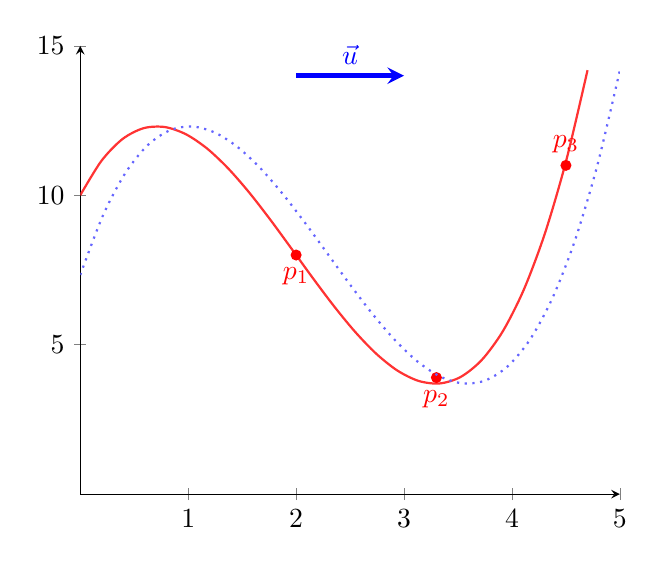
\begin{tikzpicture}
  \begin{axis} [axis lines=center,ymin=0,ymax=15,xmin=0,xmax=5]
  \draw[-stealth,ultra thick,blue] (2,14)--(3,14)node[anchor=south,midway]{$\vec{u}$};
    \addplot [domain=0:4.7, smooth, thick,red!80] { (x-2)^3 - 5*(x-2) +8};
    %\fill[red] (0.8,12.4) circle[radius=2pt] ++(0,0.1) node[anchor=south] {$p_0$};\pause   
    \fill[red] (2,8) circle[radius=2pt] ++(0,-0.1) node[anchor=north] {$p_1$};%\pause  
    \fill[red] (3.3,3.9) circle[radius=2pt] ++(0,-0.1) node[anchor=north] {$p_2$};%\pause
    \fill[red] (4.5,11) circle[radius=2pt] ++(0,0.1) node[anchor=south] {$p_3$};%\pause   
    
    \addplot [domain=0:5, smooth, thick,dotted,blue!60] { (x-2.3)^3 - 5*(x-2.3) +8};
  \end{axis}
\end{tikzpicture}
\end{column}
\begin{column}{0.5\textwidth}  %%<--- here
    \begin{center}
    \Large 
    $$\begin{aligned}
    \text{  }& - \vec{u} &\quad \dfrac{\partial c}{\partial x}& =&\dfrac{\partial c}{\partial t}\\[1em]\hline
    \text{p1}&\quad(-) &\quad (\square)&\,=\,&\,(\square)\uparrow \\[0.6em]\hline
    \text{p2}&\quad(-) &\quad (\square)&\,=\,&\,(\square)\quad \\       \hline
    \text{p3}&\quad(-) &\quad (\square)&\,=\,&\,(\square)\downarrow \\[0.6em]\hline
    \end{aligned}
    $$ 
    \end{center}
    \vfill
\end{column}
\end{columns}
 
\end{frame}

\section{Mezclado turbulento}
\begin{frame}{}
        \begin{tikzpicture}[remember picture, overlay]
            \node[opacity=1.,inner sep=1pt] at (current page.center)
            {\includegraphics[width=0.98\textwidth]{img/flujo-alrededor-cilindro.jpg}};
        \end{tikzpicture}
 \footnote{tomado de \textit{An album of fluid motion}, de Milton Van Dyke.}
\end{frame}

\begin{frame}{Turbulencia}{Mezclado por turbulencia}

\textit{La turbulencia es parte del flujo no principal que experimenta variaciones abruptas, irregulares, y caóticas.}\\[0.5em]

La turbulencia produce mezclado de las especies químicas en la atmósfera.\\[0.5em]
\pause

 El mezclado debido a la turbulencia tiene naturaleza difusiva, por lo tanto aplica la \alert{Primer ley de Fick:}
 $$\boxed{J=-K\,\dfrac{\partial c }{\partial x} }$$
\pause


El flujo neto de c  (J) debido a la difusión es negativamente proporcional al gradiente de concentraciones.
\end{frame}



\begin{frame}{Mezclado turbulento}

\begin{center}
    \DiffPict
\end{center}

$$
\begin{aligned}
\Delta m   &= ({\color{blue}J_1 A }- {\color{red}J_2 A})\Delta t\\ \pause
\Delta c \Delta x \Delta y \Delta z &= (J_1 - J_2) \Delta y \Delta z\Delta t\\ \pause
\dfrac{\Delta c}{\Delta t} &= \dfrac{J_1 - J_2}{\Delta x}\\ \pause
\dfrac{\Delta c}{\Delta t}&= - \dfrac{(-K_2\frac{\partial c_2}{\partial x}) - (-K_1\frac{\partial c_1}{\partial x})}{\Delta x}\\
\end{aligned}
$$
\pause
En el límite $\Delta x\to 0$ , $\Delta t \to 0$:
\pause
    $$\dfrac{\partial c} {\partial t}=-\dfrac{\partial}{\partial x} - K\dfrac{\partial c}{\partial x}=K\dfrac{\partial^2 c}{\partial x^2}$$
\end{frame}
\begin{frame}{Intuición}{Difusión}
 \begin{columns}
 \begin{column}{0.5\textwidth}
 \begin{tikzpicture}                   
   \begin{axis} [axis lines=center,ymin=0,ymax=15,xmin=0,xmax=5]        
     \addplot [domain=0:4.7, smooth, thick,red!80] { (x-2)^3 - 5*(x-2) +8};
     \fill[red] (0.8,12.4) circle[radius=2pt] ++(0,0.1) node[anchor=south] {$p_1$};%\pause
     \fill[red] (2,8) circle[radius=2pt] ++(0,0.1) node[anchor=south] {$p_2$};%\pause
     \fill[red] (3.3,3.9) circle[radius=2pt] ++(0,-0.1) node[anchor=north] {$p_3$};%\pause
     \addplot [domain=0:5, smooth, thick,dotted,blue!60] {0.7* (x-2)^3 - 5*(x-2)*0.7 +8};          
   \end{axis}                                                                                    
 \end{tikzpicture}            
 \end{column}
 \begin{column}{0.5\textwidth}  %%<--- here
     \begin{center}
     \Large 
     $$
     \begin{aligned}
     \text{  }& K &\quad \dfrac{\partial^2 c}{\partial x^2}& =&\dfrac{\partial c}{\partial t}\\[1em]\hline
     \text{p1}\qquad& (+) &\quad (\square)&\,=\,&\,(\square)\downarrow \\[0.6em]\hline
     \text{p2}\qquad& (+) &\quad (\square)&\,=\,&(\square)\quad \\       \hline
     \text{p3}\qquad& (+) &\quad (\square)&\,=\,&\,(\square)\uparrow \\[0.6em]\hline
     \end{aligned}
     $$ 
    \end{center}
    \vfill
 \end{column}
 \end{columns}
\end{frame}

%\vfill
%\column{0.65\textwidth}

% \only<1> {\begin{block}{Química}
% $X_1 + X_2 \rightarrow X_3 $\\
% $X_1 + X_2 + M \rightarrow X_3 + M $

% $$ \dfrac{\partial [X_{i}]}{\partial t} = S_{i}\omega_r $$

% $$k_{r}[X_1][X_2] \qquad k_{r}[X_1][X_2][M] $$
% \textit{ley de Arrenius}:
% $$k_r (T) = \alpha T^\beta exp(\frac{E_a}{RT}) $$
% \end{block} }

% \only<2> { \begin{block}{Fotoquímica}
% %$$\dfrac{\partial [X_{i}]}{\partial t} = P_{i}- L_{i}[X_{i}] $$
% $AB  + h\nu \rightarrow A + B $
% $$\dfrac{\partial [AB]}{\partial t}= \sigma_{\lambda} I_{\lambda} [AB]$$
% \end{block} }

% \only<3> { \begin{block}{Deposicion húmeda}
%  \textit{scavegging fraction rate} ($\Lambda$)
% $$\Lambda=\alpha P^{\beta}$$
% donde P es la precipitación, y $\alpha$, $\beta$ son parámetros que dependen del contaminante y el mecanismo de remoción.

% \end{block}  }

% \only<4> {\begin{block}{Deposición seca}
%  para la fase gaseosa:
% $$v_{d} =\dfrac{1}{R_a+R_b +R_c}$$
% donde $R_a$ , $R_b$ y $R_c$ son las resistencias aerodinámica, de flujo cuasi-laminar y de superficie respectivamente.
% \textit{ley de Stokes}:
% $$v_d =\dfrac{C\delta g d^{2}}{18\eta}$$
% \end{block}  }
%\end{columns}
%\only<5> {$$\boxed{\dfrac{\partial C}{\partial t}=  \pm R_{Q}\pm R_{FQ}\pm R_{L} \pm R_{D}+... =\sum_{i}^{C}R_{i}} $$}


\section{Ecuación de transporte}
\begin{frame}{Ecuación de transporte}

Finalmente, si sumamos todos los procesos, la ecuación de transporte nos queda:

%    $$\boxed{\dfrac{\partial C}{\partial t}= E - u\dfrac{\partial C}{\partial x}+ K\dfrac{\partial^2C}{\partial x^2} - \lambda C
%}$$
$$
\boxed{
    \dfrac{\partial c}{\partial t}  
    =
    \underbrace{E }_{\text{Emisión}}
    -
    \underbrace{\lambda \,c}_{\text{Química}}
    -
    \underbrace{u \dfrac{\partial c}{\partial x}  }_{\text{Advección}}
    +
    \underbrace{K \dfrac{\partial^2 c}{\partial x^2} }_{\begin{smallmatrix}\text{Mezclado}\\ \text{turbulento} \end{smallmatrix}}
}
$$
% \footnote{
% En 3-dimensiones:
%\begin{equation}
%    \dfrac{\partial C}{\partial t}= E - \nabla \cdot (\vec{v}C) + K\nabla^{2}C \pm \sum_{i=1}^{C} R_{i}
%\end{equation}
%}

\vspace{1.5em}
Para cada situación va a ser necesesario definir los parámetros: $E$, $\lambda$, $u$ y $K$
\end{frame}

